%%%%%%%%%%%%%%%%%%%%%%%%%%%%%%%%%%%%%%%%%
%
% Using Diaz essay LaTeX template from:
% http://www.LaTeXTemplates.com
%
% Authors:
% Vel (vel@LaTeXTemplates.com)
% Nicolas Diaz (nsdiaz@uc.cl)
%
% License:
% CC BY-NC-SA 3.0 (http://creativecommons.org/licenses/by-nc-sa/3.0/)
%
%%%%%%%%%%%%%%%%%%%%%%%%%%%%%%%%%%%%%%%%%

% PACKAGES AND OTHER DOCUMENT CONFIGURATIONS
\documentclass[11pt]{diazessay} % Font size (can be 10pt, 11pt or 12pt)

\usepackage{listings}
\usepackage{tikz}
\usetikzlibrary{positioning}

\lstset{frame=tb,
  language=C,
  aboveskip=3mm,
  belowskip=3mm,
  showstringspaces=false,
  columns=flexible,
  basicstyle={\small\ttfamily},
  numbers=none,
  numberstyle=\tiny\color{gray},
  keywordstyle=\color{blue},
  commentstyle=\color{dkgreen},
  stringstyle=\color{mauve},
  breaklines=false,
  breakatwhitespace=false,
  tabsize=3
}

% TITLE SECTION
\title{\textbf{Diving into Linux Perf Ring Buffer}}
\author{\textbf{Leo Yan} \textit{<leo.yan@linaro.org>}} % Author and institution
\date{\today} % Date, use \date{} for no date

\def\code#1{\texttt{#1}}

%----------------------------------------------------------------------------------------

\begin{document}

\maketitle % Print the title section

% ABSTRACT AND KEYWORDS

\begin{abstract}
Linux perf ring buffer is not only used to transfer the PMU event data, it's also a fundamental mechanism for hardware tracing with Intel PT, Arm CoreSight, etc.  Therefore, the ring buffer implementation is critical and very challenge, it is required to provide high throughput, and should avoid causing any significant overload by itself for the buffer's management.

The purpose of this article is to provide a material if anyone wants to understand the internal of pref ring buffer. By diving into the details, it explains the perf ring buffer implementation and how the ring buffer is applicated in practice.
\end{abstract}

\hspace*{3.6mm}\textit{Keywords:} Linux, perf, ring buffer, throughput, profiling % Keywords
\vspace{30pt} % Vertical whitespace between the abstract and first section

% ESSAY BODY

\section*{Introduction}

Perf tool is a main stream profiling tool which is widely used in Linux community.  At the early time, it was originally designed to support CPU PMU events, like CPU cycles, cache access and misses events, etc; afterwards, it was extended to support timers, software events (E.g. Ftrace tracepoints).  Nowdays, it has integrated with the hardware trace and even can co-work with eBPF tracing.

To support these kind events, especially if developers want to record multiple events in one go, the ring buffer plays a critical role for event recording, the kernel and perf tool in the user space use the ring buffer to exchange data, and at the end stores record into data file.

The throughput is a big challenge in the implementation, particularly, from the performance pespective, it would be very interesting to know how the buffer is synchronized between user space and kernel, and how to support SMP if the buffer is shared by multiple CPUs.  This article tries to dive into these details and give out answers to cate our curiosity.

In the sequential sections, the content is arranged as:
\begin{itemize}
	\item The introduction for basic algorithm of the ring buffer;
	\item The mechanim for AUX ring buffer;
	\item At last, using Arm CoreSight as an example to explain how the ring buffer works with hardware trace.
\end{itemize}

\section*{Implementation for the ring buffer}

\subsection*{Basic algorithm}

As said in the textbook, the ring buffer should be managed by a head pointer and a tail pointer; the head pointer is manipulated by a writer and the tail pointer is updated by a reader respectively.

\begin{center}
\par
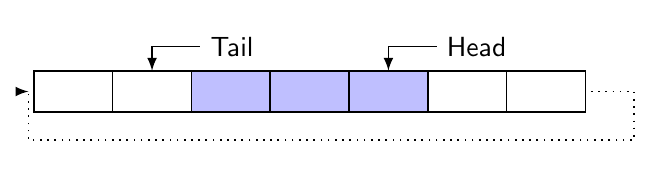
\begin{tikzpicture}[>=latex,font=\sffamily,semithick,scale=1.75]
	\centering
	\node [minimum width=1cm,minimum height=1.5em,outer sep=0pt,draw=black,fill=white] at (0,0) (A) {};
        \node [minimum width=1cm,minimum height=1.5em,outer sep=0pt,draw=black,fill=white,anchor=west] at (A.east) (B) {};
        \node [minimum width=1cm,minimum height=1.5em,outer sep=0pt,draw=black,fill=blue!25,anchor=west] at (B.east) (C) {};
        \node [minimum width=1cm,minimum height=1.5em,outer sep=0pt,draw=black,fill=blue!25,anchor=west] at (C.east) (D) {};
        \node [minimum width=1cm,minimum height=1.5em,outer sep=0pt,draw=black,fill=blue!25,anchor=west] at (D.east) (E) {};
        \node [minimum width=1cm,minimum height=1.5em,outer sep=0pt,draw=black,fill=white,anchor=west] at (E.east) (F) {};
        \node [minimum width=1cm,minimum height=1.5em,outer sep=0pt,draw=black,fill=white,anchor=west] at (F.east) (G) {};
	\draw [->,shorten >=2pt,shorten <=2pt,semithick,dotted] (G.east) -- +(1em,0em) -- +(1em,-1em) -- +(-11.5em,-1em) -- +(-11.5em,0em) -- (A.west);
	\draw [<-] (E.north) -- +(0em,.5em) -- +(1em,.5em) node [right] (Head) {Head};
	\draw [<-] (B.north) -- +(0em,.5em) -- +(1em,.5em) node [right] (Tail) {Tail};
\end{tikzpicture}

\bigskip

\par
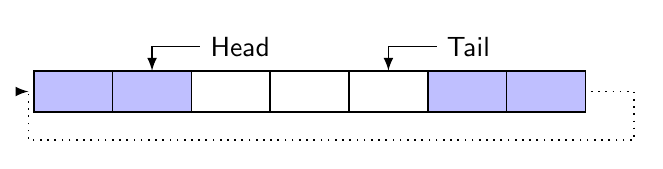
\begin{tikzpicture}[>=latex,font=\sffamily,semithick,scale=1.75]
	\node [minimum width=1cm,minimum height=1.5em,outer sep=0pt,draw=black,fill=blue!25] at (0,0) (A) {};
        \node [minimum width=1cm,minimum height=1.5em,outer sep=0pt,draw=black,fill=blue!25,anchor=west] at (A.east) (B) {};
        \node [minimum width=1cm,minimum height=1.5em,outer sep=0pt,draw=black,fill=white,anchor=west] at (B.east) (C) {};
        \node [minimum width=1cm,minimum height=1.5em,outer sep=0pt,draw=black,fill=white,anchor=west] at (C.east) (D) {};
        \node [minimum width=1cm,minimum height=1.5em,outer sep=0pt,draw=black,fill=white,anchor=west] at (D.east) (E) {};
        \node [minimum width=1cm,minimum height=1.5em,outer sep=0pt,draw=black,fill=blue!25,anchor=west] at (E.east) (F) {};
        \node [minimum width=1cm,minimum height=1.5em,outer sep=0pt,draw=black,fill=blue!25,anchor=west] at (F.east) (G) {};
	\draw [->,shorten >=2pt,shorten <=2pt,semithick,dotted] (G.east) -- +(1em,0em) -- +(1em,-1em) -- +(-11.5em,-1em) -- +(-11.5em,0em) -- (A.west);
	\draw [<-] (E.north) -- +(0em,.5em) -- +(1em,.5em) node [right] (Tail) {Tail};
	\draw [<-] (B.north) -- +(0em,.5em) -- +(1em,.5em) node [right] (Head) {Head};
\end{tikzpicture}
\par
\textbf{Figure 1: Ring buffer (without and with overflow)}
\end{center}

Similarily, perf uses the same way to manage the ring buffer.  There have two actors: a page contains the control structure for ring buffer management, and the ring buffer; following the naming convention, the page containing the control structure is named as "user page".  The user page and the ring buffer are mapped to user space via the virtual mapping area (VMA) in the continuous address space, and the user page is mapped prior to the buffer.

The control structure is defined as \code{perf\_event\_mmap\_page} which contains the head pointer \code{data\_head} and the tail pointer \code{data\_tail}.  When the kernel starting to fill records into the ring buffer, it modifies the head pointer to reserve the memory so that later can safely store events into the buffer; on the other side, the perf tool updates the tail pointer when consumes data from the ring buffer.

\begin{center}
\par
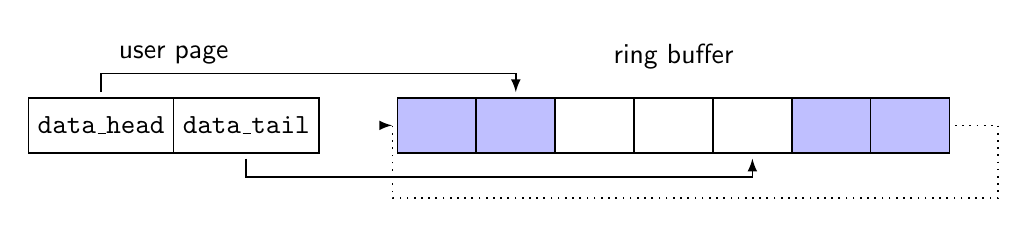
\begin{tikzpicture}[>=latex,font=\sffamily,semithick,scale=1.75]
	\node [minimum width=1cm,minimum height=2em,outer sep=0pt,draw=black,fill=white] at (0,0) (A) {\code{data\_head}};
	\node [minimum height=2em] at (A.east) (A2) {};
	\node [minimum width=1cm,minimum height=2em,outer sep=0pt,draw=black,fill=white,anchor=west] at (A.east) (B) {\code{data\_tail}};
        \node [minimum width=1cm,minimum height=2em,outer sep=0pt,draw=black,fill=blue!25,right=1cm of B] (C) {};
        \node [minimum width=1cm,minimum height=2em,outer sep=0pt,draw=black,fill=blue!25,anchor=west] at (C.east) (D) {};
        \node [minimum width=1cm,minimum height=2em,outer sep=0pt,draw=black,fill=white,anchor=west] at (D.east) (E) {};
        \node [minimum width=1cm,minimum height=2em,outer sep=0pt,draw=black,fill=white,anchor=west] at (E.east) (F) {};
        \node [minimum width=1cm,minimum height=2em,outer sep=0pt,draw=black,fill=white,anchor=west] at (F.east) (G) {};
        \node [minimum width=1cm,minimum height=2em,outer sep=0pt,draw=black,fill=blue!25,anchor=west] at (G.east) (H) {};
        \node [minimum width=1cm,minimum height=2em,outer sep=0pt,draw=black,fill=blue!25,anchor=west] at (H.east) (I) {};
	\node [minimum width=1cm,minimum height=2em,outer sep=0pt,above=0.5em of A2] (control) {user page};
	\node [minimum width=1cm,minimum height=2em,outer sep=0pt,above=0.5em of F] (buffer) {ring buffer};
	\draw [->,shorten >=2pt,shorten <=2pt,semithick,dotted] (I.east) -- +(1em,0em) -- +(1em,-1.5em) -- +(-11.5em,-1.5em) -- +(-11.5em,0em) -- (C.west);
	\draw [->,shorten >=2pt,shorten <=2pt,semithick] (A.north) -- +(0em,.5em) -| (D.north);
	\draw [->,shorten >=2pt,shorten <=2pt,semithick] (B.south) -- +(0em,-.5em) -| (G.south);
\end{tikzpicture}
\par
\textbf{Figure 2: Perf ring buffer}
\end{center}

Though the kernel allocates at once for all memory pages, including a dedicated page for the user page and the sequential pages for ring buffer, it's deferred to map the the pages to VMA area until the perf tool accesses the buffer from the user space.  In other words, the kernel event subsystem uses the linear kernel virtual address for accessing the ring buffer, the perf tool in the user space accesses the ring buffer via VMA, and at the first time accesses the buffer's page, a data abort exeception for page fault is taken and the kernel uses this occasion to map the page into VMA, thus the perf tool can continue to access the page after return back from page fault.

The function \code{perf\_mmap\_fault()} is invoked for handling page fault, which uses the function \code{perf\_mmap\_to\_page()} to figure out which page should be mapped. If \code{pg\_off} is zero it returns the pointer for the ring buffer's user page, otherwise it finds out the ring buffer's data page by using \code{pg\_off-1} as the page index (since the first page in VMA is reserved for user page, it produces offset '1' between the VMA index and data pages index).

\begin{lstlisting}
static vm_fault_t perf_mmap_fault(struct vm_fault *vmf)
{
        struct perf_event *event = vmf->vma->vm_file->private_data;
        struct perf_buffer *rb;
        vm_fault_t ret = VM_FAULT_SIGBUS;

        if (vmf->flags & FAULT_FLAG_MKWRITE) {
                if (vmf->pgoff == 0)
                        ret = 0;
                return ret;
        }

        rcu_read_lock();
        rb = rcu_dereference(event->rb);
        if (!rb)
                goto unlock;

        if (vmf->pgoff && (vmf->flags & FAULT_FLAG_WRITE))
                goto unlock;

        vmf->page = perf_mmap_to_page(rb, vmf->pgoff);
        if (!vmf->page)
                goto unlock;

        get_page(vmf->page);
        vmf->page->mapping = vmf->vma->vm_file->f_mapping;
        vmf->page->index   = vmf->pgoff;

        ret = 0;
unlock:
        rcu_read_unlock();

        return ret;
}
\end{lstlisting}

\subsection*{Ring buffer for profiling modes}

Perf profiles programs with different modes: per-thread mode, per-cpu mode, and system wide mode; the question is how the ring buffer is organized for these modes. This section describes what's exactly these modes and how the ring buffer can meet the requirement for them; at last we can review if there have any race conditions for the ring buffer caused in these modes.

For the per-thread mode, by specifying option \code{--per--thread} in perf command, the ring buffer is allocated for every profiled thread.  In this mode when the profiled thread is scheduled on a CPU, the events on that CPU will be enabled; and if the thread is cheduled out from the CPU, the events on the CPU will be disabled.  And if the thread is migrated from one CPU to another CPU, the events will be disabled on the previous CPU and enabled on the next CPU correspondingly.

\begin{center}
\par
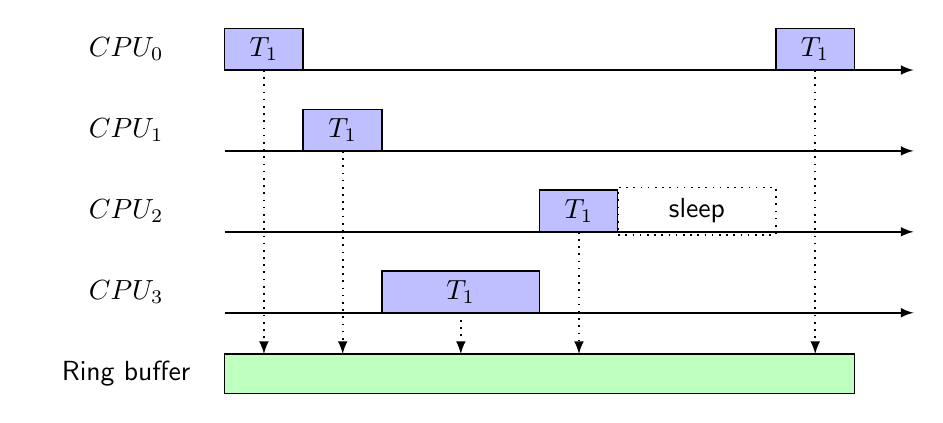
\begin{tikzpicture}[>=latex,font=\sffamily,semithick,scale=1.75]
	\node [minimum width=2.5cm,minimum height=.5cm,outer sep=0pt] at (0,0) (cpu0) {\( CPU_0 \)};
	\node [minimum width=1cm,minimum height=.5cm,outer sep=0pt,draw=black,fill=blue!25,right=0cm of cpu0] at (cpu0.east) (cpu0_p1_0) {\(T_{1}\)};
	\node [minimum width=1cm,minimum height=.5cm,outer sep=0pt,draw=black,fill=blue!25,right=7cm of cpu0] (cpu0_p1_1) {\(T_{1}\)};
	\draw[->] (cpu0.south east) -- +(5cm,0);

	\node [minimum width=2.5cm,minimum height=.5cm,outer sep=0pt,below=.5cm of cpu0] (cpu1) {\(CPU_{1}\)};
	\node [minimum width=1cm,minimum height=.5cm,outer sep=0pt,draw=black,fill=blue!25,right=1cm of cpu1] at (cpu1.east) (cpu1_p1_0) {\(T_{1}\)};
	\draw[->] (cpu1.south east) -- +(5cm,0);

	\node [minimum width=2.5cm,minimum height=.5cm,outer sep=0pt,below=.5cm of cpu1] (cpu2) {\(CPU_{2}\)};
	\node [minimum width=1cm,minimum height=.5cm,outer sep=0pt,draw=black,fill=blue!25,right=4cm of cpu2] (cpu2_p1_0) {\(T_{1}\)};
	\node [minimum width=2cm,minimum height=.6cm,outer sep=0pt,draw=black,fill=white,dotted,right=5cm of cpu2] (cpu2_p1_1) { sleep };
	\draw[->] (cpu2.south east) -- +(5cm,0);

	\node [minimum width=2.5cm,minimum height=.5cm,outer sep=0pt,below=.5cm of cpu2] (cpu3) {\(CPU_{3}\)};
	\node [minimum width=2cm,minimum height=.5cm,outer sep=0pt,draw=black,fill=blue!25,right=2cm of cpu3] (cpu3_p1_0) {\(T_{1}\)};
	\draw[->] (cpu3.south east) -- +(5cm,0);

	\node [minimum width=2.5cm,minimum height=.5cm,outer sep=0pt,below=.5cm of cpu3] (rb) {Ring buffer};
	\node [minimum width=8cm,minimum height=.5cm,outer sep=0pt,draw=black,fill=green!25,right=0cm of rb] (rb_0) {};

	\draw[->,dotted] (cpu0_p1_0.south) -- (cpu0_p1_0.south|-rb_0.north);
	\draw[->,dotted] (cpu1_p1_0.south) -- (cpu1_p1_0.south|-rb_0.north);
	\draw[->,dotted] (cpu2_p1_0.south) -- (cpu2_p1_0.south|-rb_0.north);
	\draw[->,dotted] (cpu3_p1_0.south) -- (cpu3_p1_0.south|-rb_0.north);
	\draw[->,dotted] (cpu0_p1_1.south) -- (cpu0_p1_1.south|-rb_0.north);
\end{tikzpicture}
\par
\textbf{Figure 3: Ring buffer for per-thread mode}
\end{center}

As shown in the figure 3, when perf runs in per-thread mode, a ring buffer is allocated for the profiled thread \(T_{1}\).  The ring buffer is dedicated for the thread \(T_{1}\), and no matter the thread is scheduled on any CPUs.  If the thread \(T_{1}\) is running, the perf events will be recorded into the ring buffer; during the thread's sleeping period, all associated events will be disabled, thus the ring buffer will not record any trace data anymore.


\subsection*{Writing and reading buffer}

\end{document}
